\subsection{Rangefinder Operation}
A rangefinder is a device that estimates the distance of the objects closest to it. Because this sensor suite was intended to traverse unknown locations and create a 2-dimensional map, data accuracy, precision, and reliability were vital design requirements.

\subsubsection{Selection}
The project's rangefinder selection depended on the following criteria: field of vision, maximum sensible depth, accuracy, precision, and cost. Many of the rangefinders limited by the project's budgetary restrictions were severely lacking in at least one of our project's vital criteria. However Professor Duckworth, and WPI's Electrical and Computer Engineering and Robotics Engineering Departments generously donated the URG-04LX Scanning Laser Rangefinder for the purpose of this project. The URG-04LX, shown in Figure \ref{rangefinder_pic}, is a durable, lightweight piece of equipment that has a field of view of $240^\circ$ and can sense objects up to 4 meters away with an accuracy to within 10 millimeters, which was perfect for our application \cite{urg04lx_specifications}.

\begin{figure}[H]
	\centerline{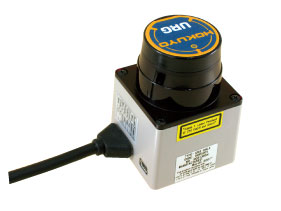
\includegraphics[width=0.5\textwidth]{urg_top.jpg}}
	\caption{URG-04LX Scanning Laser Rangefinder \cite{rangefinder_photo}}
	\label{rangefinder_pic}
\end{figure}

\subsubsection{Communication} \label{sssec:rangefinder_communication}
The URG-04LX rangefinder used the Recommend Standard (RS) 232C protocol via Universal Asynchronous Receiver/Transmitter (UART) communication. RS-232 is a form of differential serial data transmission which recognizes a digital logic high from -3V to -25V, and a digital logic low from +3V to +25V \cite{rs232}.
\par
Since the ZedBoard's Peripheral Module (Pmod) connectors supported UART communication, the rangefinder was communicated with using a Pmod IO connector. The ZedBoard's Pmod connectors used the Transistor-Transistor Logic (TTL) protocol, which is a form of non-differential serial data transmission that recognizes a logic high of +3V to +5V and a logic low of 0V \cite{ttl}. Since TTL has different logic levels than RS-232, these protocols were incompatible and did not recognize each other. Figure \ref{ttl_rs232_pic} shows a timing diagram of both RS-232 and TTL communication protocols.

\begin{figure}[H]
	\centerline{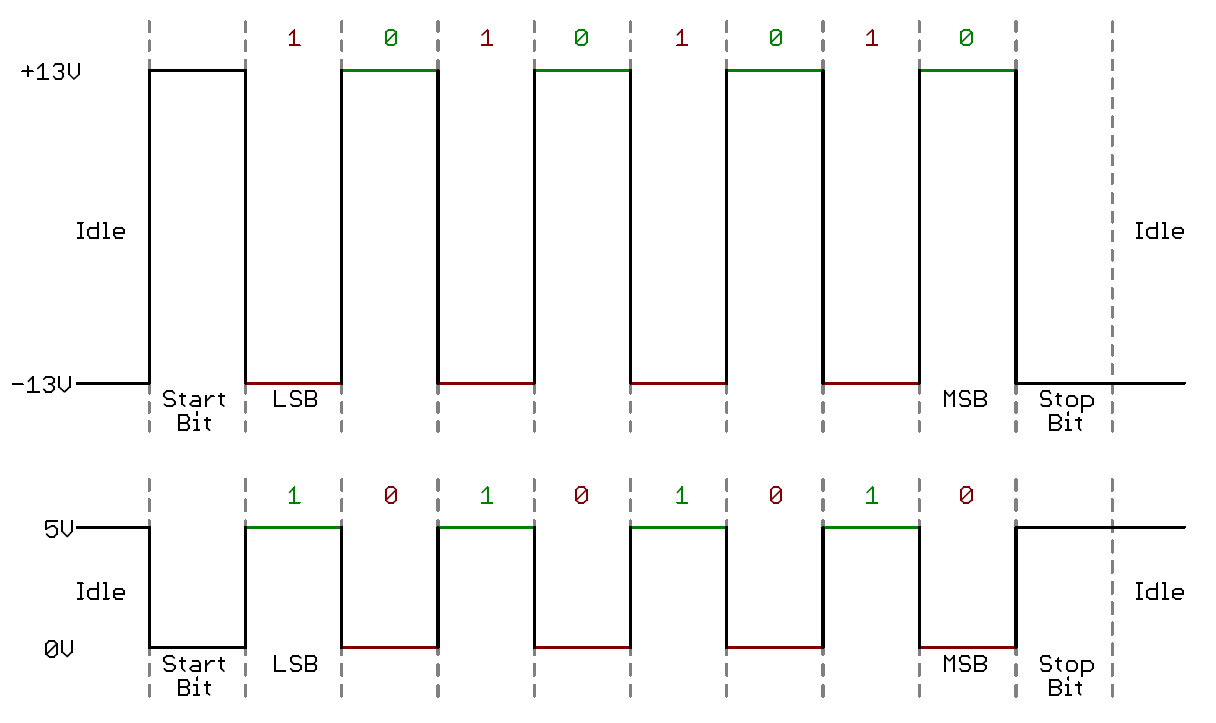
\includegraphics[width=0.9\textwidth]{ttl_rs232.png}}
	\caption{Timing Diagram of RS-232 (top) and TTL Communication Protocols \cite{ttl}}
	\label{ttl_rs232_pic}
\end{figure}

To address these logic-level issues, an external RS-232 to TTL converter board was needed to allow the rangefinder to communicate with the ZedBoard. The converter's TTL side was connected to the ZedBoard's Pmod connector, and the RS-232 side was connected to the rangefinder. For ease of connection and testing, the 9-pin DSUB RS-232 connector was connected to an RS-232 breakout board so that the pins were easily accessible. Figure \ref{rs232_ttl_breakout} shows the RS-232 to TTL converter attached to the RS-232 breakout board.

\begin{figure}[H]
	\centerline{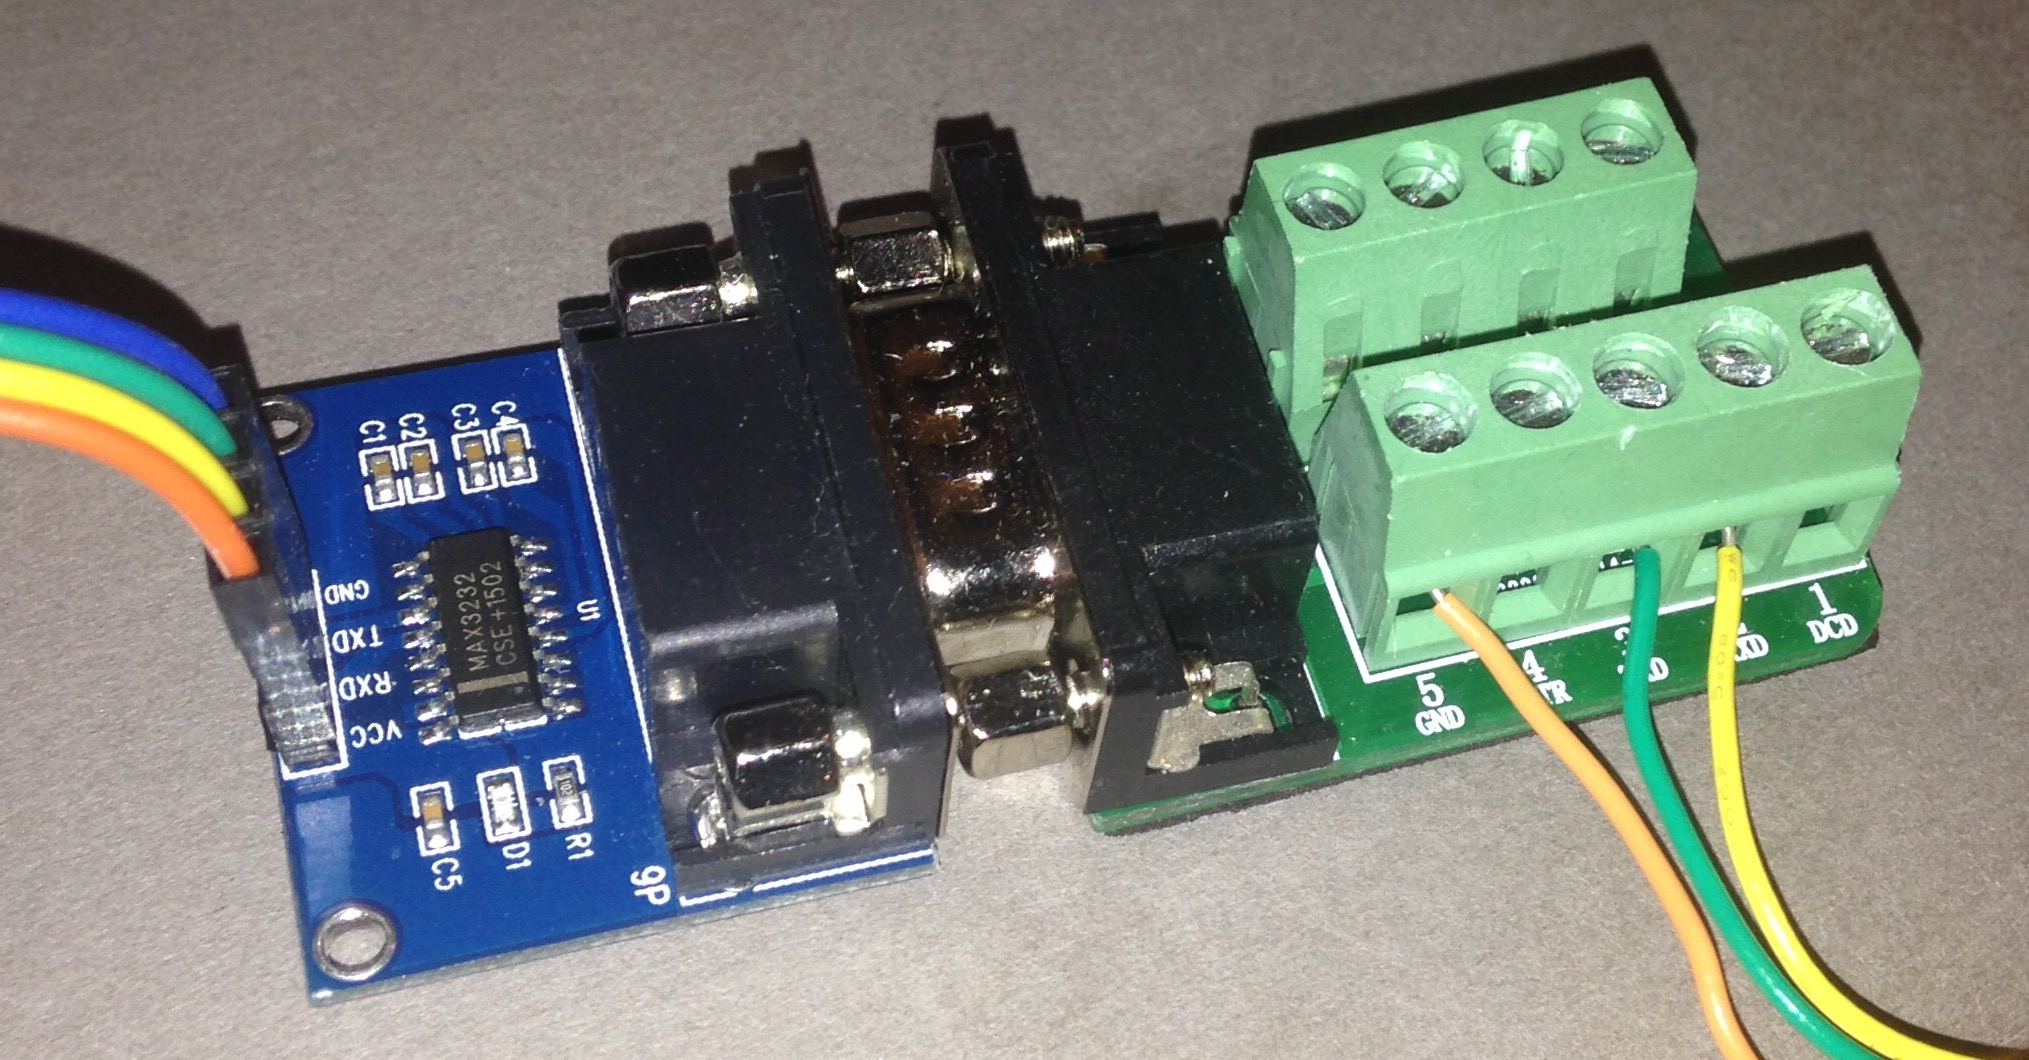
\includegraphics[width=0.6\textwidth]{rs232_ttl_breakout.png}}
	\caption{RS-232 to TTL Converter with RS-232 Breakout Board}
	\label{rs232_ttl_breakout}
\end{figure}

Although the ZedBoard's Pmod connectors were sufficient for UART communication with the URG-04LX, the power specifications were not compatible; the Pmod connectors output 3.3V but the rangefinder required 5V \cite{zedboard_datasheet, urg04lx_specifications}. Thus, the rangefinder was powered externally by a lab bench power supply.

\subsubsection{Commands}
The rangefinder defaulted to a communication speed of 19.2 kbps (19200 baud) and recognized four different commands: the version command, the communication speed setting command, the laser illumination command, and the distance data acquisition command \cite{urg04lx_datasheet}. The version command and the communication speed setting commands were both not used for the purpose of this project. The laser illumination command was used as a debugging tool to turn the laser on and off. The laser's status was displayed using a status LED on the rangefinder, so turning the laser on and off allowed for simple visual confirmation of successful communication. The distance data acquisition command was the primary command used in this project, as it was used for gathering new distance data from the rangefinder.
\par
The distance data acquisition command consisted of five different pieces that controlled the data output: 'G', the data starting point, the data end point, the cluster count, and either a line feed or a carriage return. The start point was the step of the area from where the data reading started, and the end point was where the data reading stopped. The data reading started at the start point and traversed counterclockwise until the end point. Figure \ref{rangefinder_fov} shows a top-down view of the rangefinder's field of vision with the steps labeled.

\begin{figure}[H]
	\centerline{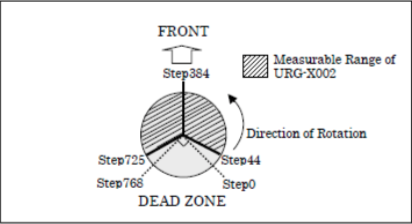
\includegraphics[width=0.7\textwidth]{rangefinder_fov.png}}
	\caption{Top-Down View of Rangefinder Field of Vision \cite{urg04lx_datasheet}}
	\label{rangefinder_fov}
\end{figure}

For this project, the beginning point was set to '000' and the end point to '768' to obtain the device's maximum coverage of $270^\circ$.
\par
The cluster count is the number of neighboring points that were grouped together as a cluster. In this implementation, the cluster count was set to '01' in order to have a cluster count of one data point.
\par
Putting all of these pieces together, the data acquisition command 'G00076801\textbackslash{}n' was obtained and transmitted from the ZedBoard to the rangefinder to request one scan of data. With the rangefinder's operation understood, an interface was created for connecting the ZedBoard to the rangefinder.




